
\chapter{矩阵}
\label{chap:matrix}

\section{向量}
\label{sec:vector}

通常$1\times n$的敌阵称为行向量,$n\times 1$的矩阵称为列向量,行向量与列向量都是向量,通常在上下文能确定是行向量还是列向量时,行列两字会省略。三维欧氏空间中的向量的点积与叉积按下式定义:
\begin{align*}
  \vec{a}\times\vec{b}\equiv
  \begin{vmatrix}
    \vec i & \vec j & \vec k\\
    a_1    & a_2    & a_3\\
    b_1    & b_2    & b_3
  \end{vmatrix}
\end{align*}


\section{行列式}
\label{sec:determinant}

行列式(Determinant)是针对$n\times n$的方阵的概念,方阵$A$的行列式通常用$\left| A\right|$或者$\det(A)$表示。二阶方阵的行列式为
\begin{align*}
  \begin{vmatrix}
    a_{11} & a_{12}\\
    a_{21} & a_{22}
  \end{vmatrix}
             \equiv a_{11}a_{22} - a_{12}a_{21}
\end{align*}

三阶方阵的行列式为
\begin{align*}
  \begin{vmatrix}
    a_{11} & a_{12} & a_{13}\\
    a_{21} & a_{22} & a_{23}\\
    a_{31} & a_{32} & a_{33}
  \end{vmatrix}\equiv
   a_{11}\begin{vmatrix} a_{22} & a_{23}\\ a_{32} & a_{33} \end{vmatrix}
  -a_{21}\begin{vmatrix} a_{12} & a_{13}\\ a_{32} & a_{33} \end{vmatrix}
  +a_{31}\begin{vmatrix} a_{12} & a_{13}\\ a_{22} & a_{23} \end{vmatrix}
\end{align*}

\begin{example}[萨吕法则,Sarrus' Rule,Sarrus' Scheme]
  将$3\times 3$的矩阵
  \begin{align*}
    M =
    \begin{pmatrix}
      a_{11} & a_{12} & a_{13}\\
      a_{21} & a_{22} & a_{23}\\
      a_{31} & a_{32} & a_{33}
    \end{pmatrix}
  \end{align*}
  按图~\ref{fig:Sarrus'-rule}扩充为$3\times 5$的矩阵并沿对角线作出辅助线:
  \begin{figure}[htbp]
    \centering
    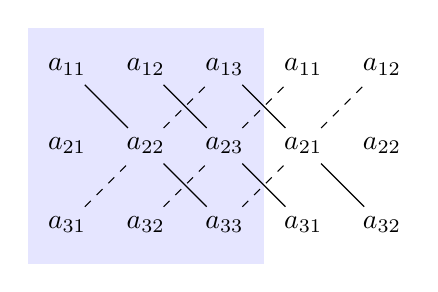
\begin{tikzpicture}[scale=1]
      \fill[color=blue!10](-.5,.5)rectangle(2.5,-2.5);
      \foreach \x/\y/\v/\i in{0/0/11/11, 1/0/12/12, 2/0/13/13, 3/0/11/e11, 4/0/12/e12,
                              0/1/21/21, 1/1/22/22, 2/1/23/23, 3/1/21/e21, 4/1/22/e22,
                              0/2/31/31, 1/2/32/32, 2/2/33/33, 3/2/31/e31, 4/2/32/e32}{
        \node(N\i) at (\x, -\y){$a_{\v}$};
      }
      \foreach \a/\b/\c in {11/22/33,12/23/e31,13/e21/e32}{
        \draw(N\a)--(N\b) (N\b)--(N\c);
      }
      \foreach \a/\b/\c in {31/22/13,32/23/e11,33/e21/e12}{
        \draw[dashed](N\a)--(N\b) (N\b)--(N\c);
      }
    \end{tikzpicture}
    \caption{萨吕法则}
    \label{fig:Sarrus'-rule}
  \end{figure}
  


  则按实线三数乘积取正,虚线三数乘积取负,然后求和,可得$\det(M)$为
  \begin{align*}
    \det(M) ={}& +a_{11}a_{22}a_{33} + a_{12}a_{23}a_{31} + a_{13}a_{21}a_{32}\\
               & -a_{31}a_{22}a_{13} + a_{32}a_{23}a_{11} - a_{33}a_{21}a_{12}
  \end{align*}
\end{example}
\begin{theorem}[三角形面积的行列式公式]
  记平面直角坐标系下三角形的3个顶点的坐标分别为$(x_1, y_1)$,$(x_2,y_2)$和$(x_3,y_3)$,则三角形的面积为
  \begin{align*}
    S =\left| \det
    \begin{pmatrix}
      x_1 & y_1 & 1\\
      x_2 & y_2 & 1\\
      x_3 & y_3 & 1
    \end{pmatrix}\right|
  \end{align*}
\end{theorem}